%% Documento gerado após muito esforço por Bruno Fernandes

\documentclass[
    % -- opções da classe memoir --
    12pt,               % tamanho da fonte
    openright,          % capítulos começam em pág ímpar (insere página vazia caso preciso)
    twoside,            % para impressão em verso e anverso. Oposto a % oneside
    a4paper,            % tamanho do papel. 
    % -- opções da classe abntex2 --
    chapter=TITLE,     % títulos de capítulos convertidos em letras maiúsculas
    %section=TITLE,     % títulos de seções convertidos em letras maiúsculas
    %subsection=TITLE,  % títulos de subseções convertidos em letras maiúsculas
    %subsubsection=TITLE,% títulos de subsubseções convertidos em letras maiúsculas
    %subsubsubsection=TITLE,% títulos de subsubsubseções convertidos em letras maiúsculas
    % -- opções do pacote babel --
    english,            % idioma adicional para hifenização
    spanish,            % idioma adicional para hifenização
    portuguese              % o último idioma é o principal do documento
    ]{abntex2} 

% ---
% Pacotes básicos 
% ---
\label{preâmbulo}

\usepackage{lmodern}            % Usa a fonte Latin Modern          
\usepackage[T1]{fontenc}        % Selecao de codigos de fonte.
\usepackage[utf8]{inputenc}     % Codificacao do documento (conversão automática dos acentos)
\usepackage{lastpage}           % Usado pela Ficha catalográfica
\usepackage{indentfirst}        % Indenta o primeiro parágrafo de cada seção.
\usepackage{color,xcolor}       % Controle das cores
\usepackage{graphicx}           % Inclusão de gráficos
\usepackage{microtype}          % para melhorias de justificação
\usepackage{booktabs}
\usepackage{tabulary}
\usepackage{caption}
\usepackage{soul}
\usepackage{rotating}

\renewenvironment{quotation}%
  {%
   \small
   \begin{list}{}{%
       \setlength{\listparindent}{0cm}%
       \setlength{\itemindent}{\listparindent}%
       \setlength{\rightmargin}{0cm}%
       \setlength{\leftmargin}{4cm}%
       \setlength{\parsep}{0pt}}%
    \item\relax}%
  {\end{list}}

\let\newfloat\undefined
\usepackage{floatrow}

\floatsetup[table]{capposition=top}
\floatsetup[figure]{capposition=top}

\captionsetup[table]{justification=centering,width=\textwidth,labelfont=bf,textfont=bf}
\captionsetup[lstlisting]{justification=centering,width=\textwidth,labelfont=bf,textfont=bf}
\captionsetup[figure]{justification=centering,width=\textwidth,labelfont=bf,textfont=bf}

	\usepackage{helvet}
	\renewcommand{\familydefault}{\sfdefault}

% ---



% ---
% Pacotes de citações
% ---

\usepackage[brazilian,hyperpageref]{backref}     % Paginas com as citações na bibl
\usepackage[alf]{abntex2cite}   % Citações padrão ABNT

% ---
% Redefinição do comando duplo quote e quote simples
% ---
\newcommand\dblquote[1]{\textquotedblleft #1\textquotedblright}
\newcommand\sglquote[1]{\textquoteleft #1\textquoteright}

% --- 
% CONFIGURAÇÕES DE PACOTES
% --- 

% ---
% Configurações do pacote backref
% Usado sem a opção hyperpageref de backref
\renewcommand{\backrefpagesname}{Citado na(s) página(s):~}
% Texto padrão antes do número das páginas
\renewcommand{\backref}{}
% Define os textos da citação
\renewcommand*{\backrefalt}[4]{
    \ifcase #1 %
        Nenhuma citação no texto.%
    \or
        Citado na página #2.%
    \else
        Citado #1 vezes nas páginas #2.%
    \fi}%
% ---


% ---
% Configurações de aparência do PDF final

% alterando o aspecto da cor azul
\definecolor{blue}{RGB}{41,5,195}

% informações do PDF
\makeatletter
\hypersetup{
        %pagebackref=true,
        pdftitle={\@title}, 
        pdfauthor={\@author},
        pdfsubject={\imprimirpreambulo},
        pdfcreator={LaTeX with abnTeX2},
        pdfkeywords={fastformat.co}, 
        %
        colorlinks=true,            % false: boxed links; true: colored links
        linkcolor=blue,             % color of internal links
        citecolor=blue,             % color of links to bibliography
        filecolor=magenta,          % color of file links
        urlcolor=blue,
        %
        bookmarksdepth=4
}
\makeatother
% --- 

% ---
% Informações de dados para CAPA e FOLHA DE ROSTO
% ---
\titulo{Estudo de como metodologias ágeis atendem boas práticas de gerenciamento de projetos de Software}

\autor{Bruno Fernandes}
\local{Maringá}
\data{Fevereiro de 2016}
\orientador{Prof. Dr. Donizete Bruzarosco}

\instituicao{
  \bfseries
  \MakeUppercase{Universidade Estadual de Maringá}
  \par
  \MakeUppercase{Departamento de Informática}
  \par
  \MakeUppercase{Bacharelado em Informática} }
\tipotrabalho{Trabalho de Conclusão de Curso}
% O preambulo deve conter o tipo do trabalho, o objetivo, 
% o nome da instituição e a área de concentração 
\preambulo{Monografia apresentada ao curso de Informática da UEM, como requisito para obtenção do título de bacharel em Informática.}
% ---

\def\volume{  }


% --- 
% Espaçamentos entre linhas e parágrafos 
% --- 

% O tamanho do parágrafo é dado por:
\setlength{\parindent}{1.3cm}

% Controle do espaçamento entre um parágrafo e outro:
\setlength{\parskip}{0.2cm}  % tente também \onelineskip

% ---
% compila o indice
% ---
\makeindex
% ---

% ----
% Início do documento
% ----
\label{inicio do doc}
\begin{document}


% Seleciona o idioma do documento (conforme pacotes do babel)
%\selectlanguage{english}
\selectlanguage{brazil}

% Retira espaço extra obsoleto entre as frases.
\frenchspacing 

% ---
\renewcommand{\ABNTEXchapterfontsize}{\LARGE}
\renewcommand{\ABNTEXpartfontsize}{\ABNTEXchapterfontsize}
\renewcommand{\ABNTEXsectionfontsize}{\Large}
\renewcommand{\ABNTEXsubsectionfontsize}{\large}
\renewcommand{\ABNTEXsubsubsectionfontsize}{\normalsize}
\renewcommand{\ABNTEXsubsubsubsectionfontsize}{\normalsize}
% ---

% ----------------------------------------------------------
% ELEMENTOS PRÉ-TEXTUAIS
% ----------------------------------------------------------
% \pretextual

% ---
% Capa
% ---
\label{capa}
\imprimircapa

% ---

% ---
% Folha de rosto
% (o * indica que haverá a ficha catalográfica)
% ---
\label{folha rosto}
\imprimirfolhaderosto*
% ---

% ---
% Inserir a ficha catalográfica
% ---
\label{ficha catalografica}
\begin{fichacatalografica}
	\sffamily
  \vspace*{10cm} 		% Posição vertical
  \hrule				% Linha horizontal
  \begin{center}		% Minipage Centralizado
  \begin{minipage}[c]{12.5cm} % Largura

  \imprimirautor

  \hspace{0.5cm} \imprimirtitulo / \imprimirautor. --
  \imprimirlocal, \imprimirdata-
  
  \hspace{0.5cm} \pageref{LastPage} p. : il.(alguma color.); 30 cm.\\

  \hspace{0.5cm} \imprimirorientadorRotulo ~\imprimirorientador\\

\hspace{0.5cm}
\parbox[t]{\textwidth}{\imprimirtipotrabalho~--~\imprimirinstituicao,
\imprimirdata.}\\

  \hspace{0.5cm}
	1. Palavra-chave1.
	2. Palavra-chave2.
	I. Orientador.
	II. Universidade xxx.
	III. Faculdade de xxx.
	IV. Título\\
	
  \hspace{8.75cm} CDU 02:141:005.7\\
  
  \end{minipage}
  \end{center}
  \hrule
  \newpage
\end{fichacatalografica}
% ---

% ---
% Inserir errata
% ---
\label{errata}
% \begin{errata}
% Elemento opcional da \citeonline[4.2.1.2]{NBR14724:2011}. Exemplo:
% 
% \vspace{\onelineskip}
% 
% FERRIGNO, C. R. A. \textbf{Tratamento de neoplasias ósseas apendiculares com
% reimplantação de enxerto ósseo autólogo autoclavado associado ao plasma
% rico em plaquetas}: estudo crítico na cirurgia de preservação de membro em
% cães. 2011. 128 f. Tese (Livre-Docência) - Faculdade de Medicina Veterinária e
% Zootecnia, Universidade de São Paulo, São Paulo, 2011.
% 
% \begin{table}[htb]
% \center
% \footnotesize
% \begin{tabular}{|p{1.4cm}|p{1cm}|p{3cm}|p{3cm}|}
%   \hline
%    \textbf{Folha} & \textbf{Linha}  & \textbf{Onde se lê}  & \textbf{Leia-se}  \\
%     \hline
%     1 & 10 & auto-conclavo & autoconclavo\\
%    \hline
% \end{tabular}
% \end{table}
% 
% \end{errata}
% ---

% ---
% Inserir folha de aprovação
% Substituir por versão digitalizada ao finalizar o TCC
% ---
\label{folha aprovação}
\begin{folhadeaprovacao}

  \begin{center}
    {\ABNTEXchapterfont\large\imprimirautor}

    \vspace*{\fill}\vspace*{\fill}
    \begin{center}
     \ABNTEXchapterfont\bfseries\Large\imprimirtitulo
    \end{center} 
    \vspace*{\fill}
    
    \hspace{.45\textwidth}
    \begin{minipage}{.5\textwidth}
        \imprimirpreambulo
    \end{minipage}%
    \vspace*{\fill}
   \end{center}
    
   Trabalho aprovado. \imprimirlocal, 24 de novembro de 2015:

   \assinatura{\textbf{\imprimirorientador} \\ Orientador} 
   \assinatura{\textbf{Professor} \\ Convidado 1}
   \assinatura{\textbf{Professor} \\ Convidado 2}
   \assinatura{\textbf{Professor} \\ Convidado 3}
      
   \begin{center}
    \vspace*{0.5cm}
    {\large\imprimirlocal}
    \par
    {\large\imprimirdata}
    \vspace*{1cm}
  \end{center}
  
\end{folhadeaprovacao}
% ---

% ---
% Dedicatória
% ---

% ---

% ---
% Agradecimentos
% --

% ---

% ---
% Epígrafe
% ---

% ---

% ---
% RESUMOS
% ---
% resumo em português


% resumo em inglês


% resumo em francês 


% resumo em espanhol

% ---

% ---
% inserir lista de ilustrações
% ---
\label{lista ilustrações}
  \pdfbookmark[0]{\listfigurename}{lof}
  \listoffigures*
  \cleardoublepage

% ---

% ---
% inserir lista de tabelas
% ---
\label{lista tabelas}
  \pdfbookmark[0]{\listtablename}{lot}
  \listoftables*
  \cleardoublepage

% ---

% ---
% inserir lista de abreviaturas e siglas
% ---
\label{lista siglas}
\begin{siglas}
	\item[ABNT] Associação Brasileira de Normas Técnicas
	\item[MPEs] Micro e Pequenas Empresas
	\item[PMBOK] Project Management Body of Knowledge
	\item[PMI] Project Management Institute
	\item[XP] eXtreme Programming

\end{siglas}

% ---
% inserir lista de símbolos
% ---
% \begin{simbolos}
%   \item[$ \Gamma $] Letra grega Gama
%   \item[$ \Lambda $] Lambda
%   \item[$ \zeta $] Letra grega minúscula zeta
%   \item[$ \in $] Pertence
% \end{simbolos}
% ---

% ---
% inserir o sumario
% ---
\tableofcontents
% ---

% ----------------------------------------------------------
% ELEMENTOS TEXTUAIS
% ----------------------------------------------------------
\textual


\chapter{Introdução}

Desenvolvimento de software não é uma tarefa trivial, principalmente quando envolve muitas pessoas trabalhando por um tempo relativamente longo. Por isto é importante que se faça um gerenciamento do projeto de desenvolvimento para que o produto final seja entregue com qualidade, no prazo e dentro do orçamento \cite[p.~555]{pressman2011}.

O \citeonline{standish2013}, através do relatório Chaos, define algumas características para projetos bem sucedidos, e são elas: projeto finalizado dentro do prazo, dentro do orçamento e contemplando todas as funcionalidades inicialmente especificadas. Neste contexto, a gerência de projetos se caracteriza como uma atividade fundamental para obtenção da qualidade do produto de software e do seu sucesso.

Para guiar o gerente de projetos no ciclo de vida do projeto, foi criado o PMBOK\index{PMBOK}, que é um conjunto de boas práticas de gerência de projetos consolidado e que hoje é aceito internacionalmente. Porém, atualmente tem sido notável a utilização de outras metodologias para gerência de projetos de software, conhecidas como metodologias ágeis. Estes modelos ditos ágeis priorizam o valor agregado e as interações entre as pessoas do que o cumprimento de prazos custo ou atendimento ao escopo inicial \cite[p.~xxi]{prikladnickiAtAll}.

As micro e pequenas empresas (MPEs) são uma parcela significativa das empresas nacionais, representando 91,2\% das empresas ativas no país \cite{ibpt2016}, porém, possuem restrições de recursos, já que as empresas enquadradas em micro e pequenas empresas são aquelas que tem faturamento bruto anual de até R\$ 3.600.000,00 \cite{brasil2006}. Esta categoria de empresas é grande usuária dos métodos ágeis e por suas limitações, possuem dificuldades para analisar se as práticas de gerência de projeto de metodologias ágeis são suficientes aos seus projetos.

Diante do cenário apresentado, surge a questão de como as práticas de gerência, orientadas por métodos ágeis, atendem a boas práticas de gerência de projeto, tais como as indicadas pelo PMBOK\index{PMBOK}, que são reconhecidas internacionalmente pela sua eficiência. Assim, o presente trabalho busca responder a esta questão, por meio de um mapeamento  entre as práticas e sua análise. Com isso, pretende-se contribuir na escolha de uma metodologia ágil que melhor atenda a boas práticas de gerência de projetos, mostrando o seu nível de atendimento.


\section{Objetivos}

\subsection{Objetivo Geral}

Este trabalho tem como objetivo geral analisar práticas de gerência de projetos orientadas por métodos ágeis mais utilizados e verificar como atendem boas práticas de gerência de projetos indicadas pelo PMBOK.

\subsection{Objetivos Específicos}
Como objetivos específicos têm-se:
\begin{alineas}
	\item Estudar as orientações do guia PMBOK para gerência de projetos.
	\item Estudar as principais metodologias ágeis atualmente utilizadas no mercado de trabalho.
	\item Relacionar as práticas das metodologias ágeis com as práticas do PMBOK.
	\item Analisar o mapeamento realizado entre as práticas
	\item Avaliação da análise comparativa feita por profissionais da empresa Benner
\end{alineas}

\section{Justificativas}

A gerência de projetos se caracteriza como uma atividade fundamental para obtenção da qualidade do produto de software e do seu sucesso. O PMBOK é um conjunto de boas práticas de gerência de projetos consolidado e aceito internacionalmente.

Os métodos ágeis estão sendo largamente utilizados por desenvolvedores de software, principalmente das MPEs, e se destacam por práticas simplificadas de desenvolvimento de software. Porém, surge a questão, se suas orientações para a gerência de projetos atendem as boas práticas indicadas pelo PMBOK.

Assim, esta pesquisa visa analisar tais fatos, contribuindo com esclarecimentos sobre os mesmos, para auxiliar desenvolvedores de software para uma gerência efetiva de desenvolvimento de software.


\section{Metodologia}

Para o desenvolvimento do presente trabalho serão utilizados os seguintes recursos:
\begin{alineas}
	\item Normas ABNT para desenvolvimento de trabalhos científicos
	\item Guia PMBOK 5ª edição em Português
	\item Computador com sistema operacional Linux tendo instalado o \LaTeX \ e o editor Texmaker
	\item Empresa Benner como case para avaliar a análise comparativa realizada
\end{alineas}


Além dos recursos utilizados, não menos importante para o desenvolvimento deste trabalho, são as seguintes etapas: 

\begin{alineas}	
	\item Revisão bibliográfica: os conceitos envolvidos com o tema do trabalho são descritos, a partir de pesquisa realizada em livros, artigos, teses, dissertações, etc, atualizados, bem como é feito um levantamento de trabalhos relacionados.
	\item Análise das práticas do PMBOK: é feita uma síntese das práticas sugeridas pelo PMBOK para gerenciamento de projetos, e descrito como estas práticas se aplicam ao gerenciamento de projetos de software.
	\item Análise do ciclo de vida do XP e suas práticas de gerência: serão analisadas e descritas as práticas de gerenciamento de projeto do XP, uma metodologia de desenvolvimento ágil. Neste capítulo será mostrado todo o ciclo de vida do XP e como ele propõe que o gerenciamento do projeto seja realizado a fim de atingir a qualidade do software.
	\item Análise do ciclo de vida do Scrum e suas práticas de gerência: Assim como no capítulo anterior, será descrito detalhadamente como o Scrum se propõe a trazer qualidade com qualidade ao software produzido. Será feita uma análise do Scrum aplicado apenas ao desenvolvimento de software e não a projetos gerais, mesmo que o Scrum não se limite a este escopo.
	\item Mapeamento entre as práticas de gerência: neste capítulo selecionaremos as atividades e práticas de gerenciamento de projetos e iremos mostrá-las, através de tabelas para comparação. As atividades e práticas listadas serão as definidas pelo PMBOK, XP e Scrum.
	\item Análise do mapeamento: tendo o mapeamento das práticas de gerenciamento de projetos feito, analisaremos, de forma qualitativa, como o as práticas do XP e do Scrum atendem as boas práticas de gerenciamento de projetos de software. Não será realizada uma análise quantitativa, pois entendemos que algumas práticas podem compensar outras, mesmo não tendo a mesma nomenclatura ou artefato resultante.
	\item Avaliação da análise comparativa realizada, por profissionais da área da empresa Benner: será realizado um questionário com profissionais da empresa Benner. Estas pessoas, preferencialmente, serão pessoas com vivência, ou experiência em métodos tradicionais e ágeis de desenvolvimento de software para que possamos ter uma visão mais ampla das diferenças e semelhanças entre as práticas ágeis e tradicionais.
	\item Conclusão: Nesta fase do trabalho iremos resgatar a relevância de projetos de software e responder, finalmente, à pergunta inicialmente feita: As metodologias ágeis desenvolvimento de software atendem boas práticas de gerenciamento de projetos? Também serão apresentadas as considerações dos resultados, as dificuldades enfrentadas, as contribuições deste trabalho e propostos trabalhos futuros.
\end{alineas}

\section{Estrutura do Trabalho}
No capítulo 2 a gerência de projetos  é contextualizada na Engenharia de Software, bem como é apresentada a origem das principais metodologias utilizadas atualmente para o desenvolvimento de software. Também é mostrada uma síntese das práticas do PMBOK e o ciclo de vida dos dois métodos ágeis mais utilizados. Finalmente, são descritas as principais características de uma MPE e suas restrições.

No capítulo 3, o conhecimento adquirido no referencial teórico é utilizado para criar um mapeamento entre as práticas de gerência de projetos dos métodos ágeis XP/Scrum e do PMBOK.

No capítulo 4, é feita a análise do mapeamento realizado no capítulo anterior, destacando as diferenças entre as práticas.

No capítulo 5, é resgatada a relevância da gerência de projetos de software e indicados como os objetivos deste trabalho são atendidos. Também são apresentados as considerações de seus resultados, as dificuldades enfrentadas, as contribuições e trabalhos futuros.

\chapter{Engenharia de Software com abordagem em gerência de projetos}

De acordo com o \textit{Project Management Institute} \cite{pmi2013}, projeto\index{Projeto} é \dblquote{um esforço temporário empreendido para criar um produto, serviço ou resultado único}. Temporário porque um projeto precisa ter começo e fim definidos e único pois deve ser, de alguma forma, diferente de todos os produtos, serviços e resultados semelhantes. Adicionando-se à isto, um projeto possui limite de financiamento, ou orçamento, e consome recursos humanos e não humanos, ou seja, dinheiro, pessoas, máquinas, entre outros \cite[p.~2]{kerzner2011}. É importante salientar, também, o que não é um projeto. \dblquote{Projetos não devem ser confundidos com o trabalho diário. Um projeto não é rotineiro nem repetitivo} \cite[p.~6]{grayLarson2009}.

No Brasil existem dois termos parecidos, mas com sentidos diferentes e que não devem ser confundidos:

\begin{alineas}
	\item Projeto de Software;
	\item Projeto de desenvolvimento de Software.
\end{alineas}

O primeiro é o \textit{Software Design}, em inglês, ou seja, é um processo iterativo por meio do qual os requisitos são traduzidos em um \dblquote{documento} para construção do software. O segundo, do qual se trata o presente trabalho, vem do inglês \textit{Project}, que é de fato o esforço para criação de um produto, serviço ou resultado único. Projeto (\textit{Project}) não está relacionado apenas a Softwares. Podem ser aplicados às várias áreas de conhecimento humano \cite{pressman2006}.

Para que um projeto obtenha sucesso é altamente recomendado que haja um acompanhamento, ou gerenciamento do projeto. Segundo o \citeonline{pmi2013}, Gerenciamento de Projetos é \dblquote{a aplicação de conhecimentos, habilidades, ferramentas e técnicas às atividades do projeto a fim de atender aos seus requisitos}. Gerenciamento de projetos também é um estilo de administração orientado a resultados que premia a criação de relacionamentos colaborativos entre as diferentes pessoas de uma equipe \cite[p.~3]{grayLarson2009}.

Os conceitos acima se aplicam a projetos de diversas áreas, mas projetos de desenvolvimento de software podem ser definidos, também, como um esforço envolvendo planejamento monitoração e controle de pessoas, processos e eventos que ocorrendo à medida que o software evolui, desde os conceitos preliminares, até sua, completa e operacional, disponibilização \cite{pressman2011}. Projetos de desenvolvimento de software possuem algumas características distintas de outros projetos que podem fazer com que esse seja particularmente desafiador. Segundo \citeonline[p.~60]{sommerville2011}, algumas dessas diferenças são:

\begin{alineas}
	\item O produto é intangível. O software não pode ser visto ou tocado, deste modo, não há como o gerente de projetos saber o progresso do projeto apenas olhando para o artefato que está sendo construído.
	\item Geralmente, os grandes projetos de softwares são diferentes dos projetos anteriores em algum aspecto. Somando-se a isto o fato da tecnologia em computadores evoluir muito rapidamente, mesmo gerentes de projetos com grande experiência podem achar difícil antecipar problemas e transferir lições aprendidas para novos projetos.
	\item Os processos de software são variáveis e de organização específica. Embora tenhamos tido grande progresso na padronização e melhorias dos processo, ainda não podemos dizer com certeza quando um processo irá levar a problemas de desenvolvimento, principalmente quando o projeto de software faz parte de um projeto de engenharia de sistemas mais amplo.
\end{alineas}

Segundo \citeonline[p.~5]{grayLarson2009}, o maior objetivo de um projeto de desenvolvimento de software, assim como a maioria dos esforços de uma organização, é a satisfação de um cliente. Mas existem 5 principais características de um projeto, que o diferencia de outros esforços da Organização: 

\begin{alineas}
	\item possui objetivo estabelecido;
	\item possui período de validade definido;
	\item geralmente conta com o envolvimento de diversos departamentos e profissionais;
	\item comumente é para a elaboração de algo nunca antes realizado;
	\item possui tempo, custo e requerimentos de desempenho específicos.
\end{alineas}

Para \citeonline[p.~11]{Cruz2013}, a obtenção do objetivo é alcançada quando o gerenciamento de projetos contempla pelo menos os seguintes itens:

\begin{alineas}
	\item identificação dos requisitos;
	\item adaptação às diferentes expectativas das partes e às mudanças ao longo do ciclo de vida; e
	\item balanceamento adequado às restrições do projeto (Escopo, Qualidade, Cronograma, Orçamento, Recursos e Riscos).
\end{alineas}

Os fundamentos do gerenciamento ágil de software são o Manifesto Ágil e a Declaração de Interdependência.
O manifesto ágil, como ficou conhecido, foi rascunhado em 2001 por um grupo de especialistas que disseram estar descobrindo maneiras melhores de desenvolver software valorizando os itens abaixo:

\begin{citacao}
\textbf{Indivíduos e interações} mais que processos e ferramentas \newline
\textbf{Software em funcionamento} mais que documentação abrangente \newline
\textbf{Colaboração com o cliente} mais que negociação de contratos \newline
\textbf{Responder a mudanças} mais que seguir um plano \cite{manifesto2001}.
\end{citacao}

Porém, ao contrário do que muitos pensam, o desenvolvimento ágil não deve abandonar os itens à direita, mas valorizar mais os itens da esquerda \cite{manifesto2001}.

\section{Gerente de Projetos}
O gerente de projetos é a pessoa designada para liderar a equipe responsável por alcançar os objetivos do projeto \cite[p.~16]{pmi2013}. Segundo \citeonline[p.~485]{pressman2006} o Gerente de projetos é responsável por planejar, motivar, organizar e controlar os profissionais que fazem o trabalho de software.

Segundo o \citeonline{pmi2013} para que o gerente de projetos seja eficiente e eficaz, além de possuir habilidades na área específica do projeto em que está atuando, é desejável que também possua as seguintes competências:

\begin{alineas}
	\item conhecimento sobre gerenciamento de projetos;
	\item capacidade de fazer ou realizar algo quando aplica seus conhecimentos em gerenciamento de projetos ;
	\item comportamento gerencial e características de personalidade que fornecem a habilidade de guiar a equipe do projeto para se atingir os objetivos e equilibrar as restrições do projeto.
\end{alineas}

Ainda segundo o \citeonline{pmi2013}, o gerente de projetos deve possuir uma combinação equilibrada de habilidades éticas, interpessoais e conceituais para ajudá-los a analisar situações e agir de maneira apropriada:

\begin{alineas}
	\item liderança;
	\item construção de equipes;
	\item motivação;
	\item comunicação;
	\item influência;
	\item poder de decisão;
	\item consciência política e cultural;
	\item negociação;
	\item construção de confiança;
	\item gerenciamento de conflitos;
	\item \textit{coaching}.
\end{alineas}

Para \citeonline[p.~9]{kerzner2011}, dentre as habilidades desejadas para o Gerente de Projetos, as mais importantes não são as habilidades técnicas, mas sim as pessoais. O Gerente de projetos precisa conhecer sobre psicologia, comportamento humano e organizacional, relacionamento interpessoal e comunicação. Os Gerentes de projetos geralmente possuem grandes responsabilidades, mas pouca autoridade. Assim, precisam estar sempre negociando com a alta administração e gerências funcionais.

O trabalho do Gerente de projetos varia bastante, de acordo com a organização e o produto que está sendo desenvolvido. Mas para \citeonline{sommerville2011}, a maioria dos gerentes de projetos assumem, em algum momento, responsabilidade por algumas atividades bases comuns. O planejamento do projeto é uma destas atividades, onde o gerente deve garantir que o trabalho esteja sendo feito conforme os padrões e devendo acompanhar o progresso para garantir que o desenvolvimento está no prazo e dentro do orçamento. Também é responsável por fazer a ponte entre o desenvolvimento e os clientes e gerentes da empresa, mostrando o andamento do projeto de forma concisa e coerente, abstraindo as informações mais técnicas. Os gerenciamentos de riscos e pessoas são outras atividades desempenhadas em algum momento pelos gerentes de projetos. Eles devem ser capazes de avaliar e controlar os riscos que podem afetar o projeto e agir quando necessário, bem como estabelecer formas de trabalho que levem a um desempenho eficaz da equipe. Por fim, os gerentes devem ser capazes de elaborar propostas, descrevendo os objetivos do projeto e como ele será realizado, visando ganhar um contrato para executar um item de trabalho.

\section{Ciclo de vida do projeto}
Para compreender o gerenciamento de projetos é importante conhecer seu ciclo de vida. Segundo o \citeonline[p.~38]{pmi2013}, ciclo de vida do projeto é a serie de fases pelas quais o projeto passa, desde seu início até o término. As etapas entre a inicialização e a finalização do projeto podem ser sequenciais, iterativas ou sobrepostas e estas etapas são definidas ou moldadas conforme a necessidade de gerenciamento da organização. Independentemente dos moldes utilizados pelas empresas, todos os projetos possuem início e fim definidos e as fases podem ser desmembradas em entregas ou resultados intermediários.

Apesar de variar em tamanho e complexidade, todos os projetos podem ser mapeados para a estrutura de ciclo de vida a seguir \cite[p.~39]{pmi2013}:

\begin{alineas}
	\item início do projeto;
	\item organização e preparação;
	\item execução do trabalho do projeto;
	\item encerramento do projeto;
\end{alineas}

A estrutura acima e seu desenvolvimento ao londo do tempo pode ser ilustrada pela Figura~\ref{fig:ciclo_vida_projeto}, que mostra o nível de esforço e custo de cada fase.

\begin{figure}[htb]
\RawFloats
	\caption{\label{fig:ciclo_vida_projeto}Ciclo de vida de projetos (estrutura básica)}
	\begin{center}
	    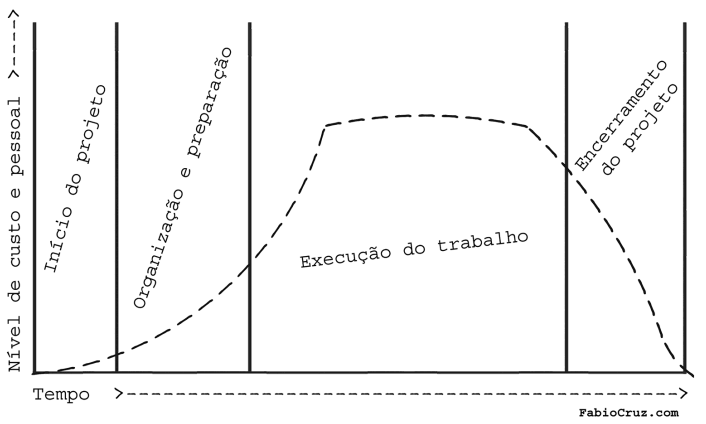
\includegraphics[scale=0.50]{figuras/ciclo_vida_projeto.png}
	\end{center}
	\legend{Fonte: \cite[p.~13]{Cruz2013}}
\end{figure}

A partir desta estrutura básica, o projeto pode ser dividido em fases, que irão proporcionar benefícios ao trabalho que será feito para se atingir os objetivos do projeto. O ciclo de vida de projetos possuem cinco fases claras, segundo o PMBOK. Estas fases, também chamadas Grupos de Processos, são bem definidas e sequenciais, possuem passos a serem executados e são conhecidas por Iniciação, Planejamento, Execução, Monitoramento e Controle e Encerramento \cite[p.~14]{Cruz2013}. 

A Figura~\ref{fig:grupo_processos} mostra a interação entre cada um dos grupos de processo ao longo do ciclo de vida do projeto e o esforço empreendido, onde as curvas mais acentuadas denotam maior importância no período \cite[p.~15]{Rafael2012}. 

\begin{figure}[htb]
\RawFloats
	\caption{\label{fig:grupo_processos}Interação entre os grupos de processos do PMBOK}
	\begin{center}
	    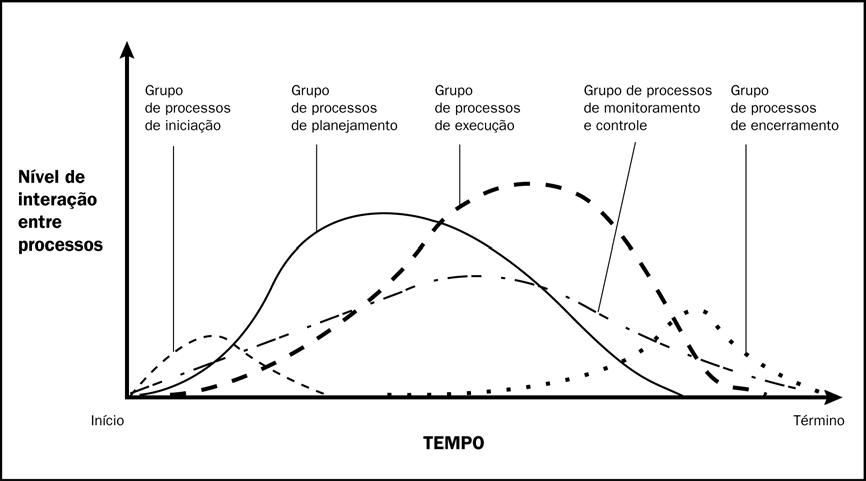
\includegraphics[scale=0.50]{figuras/grupos_processos.jpg}
	\end{center}
	\legend{Fonte: \cite[p.~51]{pmi2013}}
\end{figure}

\subsection{Iniciação}
A fase de inicialização do projeto é quando a autorização para o início de um novo projeto, ou nova fase de um projeto é obtida, o escopo inicial é definido, os recursos financeiros iniciais são comprometidos, os interessados internos e externos são identificados e o Gerente de projeto é definido. O objetivo principal desta fase é alinhar as expectativas das partes interessadas com os objetivos do projeto, dar-lhes visibilidade sobre o escopo e objetivos, e mostrar como a sua participação no projeto irá contribuir para que as expectativas sejam atingidas \cite[p.~54]{pmi2013}.

\subsection{Planejamento}
Neste grupo de processos estão os processos realizados para estabelecer o escopo, definir e refinar objetivos e desenvolver o curso de ações necessário para se atingir estes objetivos. O principal benefício deste grupo de processos é delinear a estratégia e a tática, e também o caminho para a conclusão do projeto com sucesso. O planejamento explorará as seguintes áreas apresentadas no Guia PMBOK: escopo, tempo, qualidade, comunicações, recursos humanos, riscos, aquisições e gerenciamento das partes interessadas \cite[p.~55]{pmi2013}.

\subsection{Execução}
Este grupo consiste dos processos executados para se concluir o trabalho definido no plano de gerenciamento do projeto. Este grupo também envolve coordenar a equipe e recursos, e gerenciar as expectativas das partes interessadas. Durante a execução do projeto podem surgir alterações com relação ao planejado e podem surgir riscos não esperados. Estas alterações são analisadas e, se necessário, o plano se de gerenciamento é alterado \cite[p.~55]{pmi2013}.

\subsection{Monitoramento e Controle}
O grupo de monitoramento e controle consiste dos processos necessários para acompanhar e analisar o andamento e o desempenho do projeto. O principal benefício deste grupo é a medição e análise do desempenho do projeto com o objetivo de identificar variações no plano de gerenciamento do projeto. Este controle fornece à equipe uma visão melhor do andamento do projeto e identifica as áreas que precisam de mais atenção \cite[p.~55]{pmi2013}.

\subsection{Encerramento}
Os processos deste grupo tem a finalidade de encerrar todas as atividades de todos os grupos de processos de gerenciamento do projeto, assim finalizado formalmente o projeto, as fases ou as obrigações contratuais. Este grupo de processo verifica se os processos definidos estão completos em todos os grupos de processos. Este grupo também formaliza encerramentos prematuros do projeto, como por exemplo, projetos abortados \cite[p.~55]{pmi2013}.


	
\chapter{Cronograma}

\begin{table}[h]
\centering
\begin{tabular}{|l|l|l|l|l|l|l|l|l|} \hline
ATIVIDADES                             &JUN & JUL & AGO & SET & OUT & NOV & DEZ & JAN  \\ \hline\hline
Revisão bibliográfica                  &\ \ X &\ \ X &   &     &     &     &     &     \\ \hline
Análise das práticas do PMBOK          &     &     &\ \ X &    &     &     &     &     \\ \hline
Análise do ciclo de vida do XP e 	   &	 &	   &	 &	   &	 &	   &	 &	    \\
suas práticas de gerência              &     &     &     &\ \ X &    &     &     &     \\ \hline
Análise do ciclo de vida do Scrum 	   &	 &	   &	 &	   &	 &	   &	 &      \\
e suas práticas de gerência            &     &     &     &\ \ X &    &     &     &     \\ \hline
Mapeamento entre as práticas de        &     &     &     &     &     &     &     &      \\
gerência                               &     &     &     &     &\ \ X &    &     &     \\ \hline
Análise do mapeamento                  &     &     &     &     &\ \ X &    &     &     \\ \hline
Avaliação por profissionais da área    &     &     &     &     &     &     &     &      \\
da empresa Benner, da análise          &     &     &     &     &     &\ \ X &    &     \\ 
comparativa feita                      &     &     &     &     &     &     &     &      \\ \hline
Conclusão e entrega da monografia      &     &     &     &     &     &     &\ \ X &     \\ \hline
Defesa                                 &     &     &     &     &     &     &     &\ \ X \\ \hline
Correção e entrega da monografia       &     &     &     &     &     &     &     &      \\
final                                  &     &     &     &     &     &     &     &\ \ X  \\ \hline
\end{tabular}
\end{table}


%\chapter{Resultados}

%Lorem ipsum dolor sit amet, consectetur adipisicing elit, sed do eiusmod tempor incididunt ut labore et dolore magna aliqua. Ut enim ad minim veniam, quis nostrud exercitation ullamco laboris nisi ut aliquip ex ea commodo consequat. Duis aute irure dolor in reprehenderit in voluptate velit esse cillum dolore eu fugiat nulla pariatur. Excepteur sint occaecat cupidatat non proident, sunt in culpa qui officia deserunt mollit anim id est laborum.


%\chapter{Conclusão}

%Lorem ipsum dolor sit amet, consectetur adipisicing elit, sed do eiusmod tempor incididunt ut labore et dolore magna aliqua. Ut enim ad minim veniam, quis nostrud exercitation ullamco laboris nisi ut aliquip ex ea commodo consequat. Duis aute irure dolor in reprehenderit in voluptate velit esse cillum dolore eu fugiat nulla pariatur. Excepteur sint occaecat cupidatat non proident, sunt in culpa qui officia deserunt mollit anim id est laborum.



% ----------------------------------------------------------
% ELEMENTOS PÓS-TEXTUAIS
% ----------------------------------------------------------
\postextual
% ----------------------------------------------------------

% ----------------------------------------------------------
% Referências bibliográficas
% ----------------------------------------------------------
\bibliography{references}



% ----------------------------------------------------------
% Glossário
% ----------------------------------------------------------
%
% Consulte o manual da classe abntex2 para orientações sobre o glossário.
%
%\glossary

% ----------------------------------------------------------
% Apêndices
% ----------------------------------------------------------

% ---
% Inicia os apêndices
% ---

% ---


% ----------------------------------------------------------
% Anexos
% ----------------------------------------------------------

% ---
% Inicia os anexos
% ---


%---------------------------------------------------------------------
% INDICE REMISSIVO
%---------------------------------------------------------------------
\phantompart
\printindex
%---------------------------------------------------------------------

\end{document}